
\section{Experiments}
%\begin{table*}[t]
%\centering
%\caption{Performance comparison with different baselines on the KGQA datasets.}
%\label{tab:performance_comparison}

%\setlength{\tabcolsep}{2pt}
%\resizebox{0.95\textwidth}{!}{
%\begin{tabular}{lcccccccccc}
%\toprule
%\multirow{2}{*}{Method} & \multicolumn{2}{c}{WebQSP} & \multicolumn{2}{c}{CWQ} & \multicolumn{2}{c}{GrailQA} & \multicolumn{2}{c}{QALD} & \multicolumn{2}{c}{2Wiki} \\
%\cmidrule(lr){2-3}\cmidrule(lr){4-5}\cmidrule(lr){6-7}\cmidrule(lr){8-9}\cmidrule(lr){10-11}
% & Hit@1 & F1 & Hit@1 & F1 & Hit@1 & F1 & Hit@1 & F1 & Hit@1 & F1 \\
%\midrule
%\multicolumn{11}{l}{\textit{LLM Reasoning}} \\

%\multicolumn{11}{l}{\textit{Graph Reasoning}} \\
%KD-CoT~\cite{wang2023knowledgedrivencotexploringfaithful} & 68.6 & 52.5 & 55.7 & - & - & - & - & - & - & - \\
%EWEK-QA~\cite{dehghan2024ewekqaenhancedwebefficient} & 71.3 & - & 52.5 & - & 60.4 & - & - & - & - & - \\
%ToG~\cite{sun2023think} (ChatGPT) & 76.2 & - & 57.6 & - & 68.7 & - & 50.2 & - & - & - \\
%ToG (GPT-4) & 82.6 & - & 68.5 & - & 81.4 & - & 53.8 & - & - & - \\
%EffiQA~\cite{dong2024effiqaefficientquestionansweringstrategic} & 82.9 & - & 69.5 & - & 78.4 & - & 51.4 & - & - & - \\
%RoG~\cite{luo2024rog} (Llama-2-7B) & 85.7 & 70.8 & 62.6 & 56.2 & - & - & - & - & - & - \\
%GNN-RAG~\cite{mavromatis2024gnn}(Llama-2-7B) & 85.7 & 71.3 & 66.8 & 59.4 & - & - & - & - & - & - \\
%GNN-RAG+RA(Llama-2-7B) & 90.7 & 73.5 & 68.7 & 60.4 & - & - & - & - & - & - \\
%KG-Agent~\cite{jiang2024kgagentefficientautonomousagent}(Llama-2-7B) & 83.3 & 81.0 & 72.2 & 69.8 & - & 86.1 & - & - & - & - \\
%DoG~\cite{li-etal-2025-decoding-graphs} (bs=3, Llama-3.1-8B) & 91.38 & - & 76.16 & - & - & - & - & - & 84.06 & - \\
%GCR~\cite{luo2025graphconstrainedreasoningfaithfulreasoning} (Llama-3.1-8B + ChatGPT) & 92.6 & 78.2 & 72.7 & 60.9 & - & - & - & - & - & - \\
%GCR (Llama-3.1-8B + GPT-4o-mini) & 92.2 & 79.1 & 75.8 & 61.7 & - & - & - & - & - & - \\
%\midrule
%Gemini-2.5 Flash & 50.8 & 35.5 & 25.3 & 21.6 & - & - & - & - & - & - \\
%Gemini-2.5 Pro & 55.5 & 34.8 & 28.1 & 22.4 & - & - & - & - & - & - \\
%GPT5 & 68.5 & 38.1 & 38.5 & 28.0 & - & - & - & - & - & - \\
%\midrule
%\textbf{EOG (Qwen2.5-7B + outcome)} & 83.9 & 72.6 & 70.5 & 62.1 & 90.3 & 88.2 & 79.6 & - & 82.5 & 81.9 \\
%\textbf{EOG (Qwen2.5-7B）} & 90.7 & 78.1 & 81.9 & 71.8 & 93.6 & 90.7 & 79.6 & - & 80.3 & - \\
%\textbf{SFT (Llama-3.1-8B)} & 84.3 & 74.3 & 72.1 & 63.2 & 91.5 & 86.6 & 91.5 & 86.6 & 84.9 & 82.4 \\
%\textbf{EOG (Llama-3.1-8B)} & \textbf{92.8} & \textbf{80.7} & \textbf{84.3} & \textbf{73.9} & \textbf{96.1} & \textbf{91.6} & 96.1 & 91.6 & \textbf{85.3} & \textbf{84.3} \\
%\bottomrule
%\end{tabular} 
%}
%\end{table*}
% \begin{table*}[t]
% \centering
% \caption{Performance comparison with different baselines on the KGQA datasets.}
% \label{tab:performance_comparison}
% \setlength{\tabcolsep}{2pt}
% \resizebox{0.95\textwidth}{!}{
% \begin{tabular}{llcccccccccc}
% \toprule
% \multirow{2}{*}{Method} & \multirow{2}{*}{Models} & \multicolumn{2}{c}{WebQSP} & \multicolumn{2}{c}{CWQ} & \multicolumn{2}{c}{GrailQA} & \multicolumn{2}{c}{QALD} & \multicolumn{2}{c}{2Wiki} \\
% \cmidrule(lr){3-4}\cmidrule(lr){5-6}\cmidrule(lr){7-8}\cmidrule(lr){9-10}\cmidrule(lr){11-12}
% & & Hit@1 & F1 & Hit@1 & F1 & Hit@1 & F1 & Hit@1 & F1 & Hit@1 & F1 \\
% \midrule
% KD-CoT~\citeyear{wang2023knowledgedrivencotexploringfaithful} & - & 68.6 & 52.5 & 55.7 & - & - & - & - & - & - & - \\
% EWEK-QA~\citeyear{dehghan2024ewekqaenhancedwebefficient} & - & 71.3 & - & 52.5 & - & 60.4 & - & - & - & - & - \\
% \multirow{2}{*}{ToG~\citeyear{sun2023think}} & ChatGPT & 76.2 & - & 57.6 & - & 68.7 & - & 50.2 & - & - & - \\
% & GPT-4 & 82.6 & - & 68.5 & - & 81.4 & - & 53.8 & - & - & - \\
% EffiQA~\citeyear{dong2024effiqaefficientquestionansweringstrategic} & - & 82.9 & - & 69.5 & - & 78.4 & - & - & - & - & - \\
% RoG~\citeyear{luo2024rog} & Llama-2-7B & 85.7 & 70.8 & 62.6 & 56.2 & - & - & - & - & - & - \\
% GNN-RAG~\citeyear{mavromatis2024gnn} & Llama-2-7B & 85.7 & 71.3 & 66.8 & 59.4 & - & - & - & - & - & - \\
% KG-Agent~\citeyear{jiang2024kgagentefficientautonomousagent} & Llama-2-7B & 83.3 & 81.0 & 72.2 & 69.8 & - & 86.1 & - & - & - & - \\
% DoG~\citeyear{li-etal-2025-decoding-graphs} & Llama-3.1-8B & 91.38 & - & 76.16 & - & - & - & - & - & 84.06 & - \\
% GCR~\citeyear{luo2025graphconstrainedreasoningfaithfulreasoning} 
% & Llama-3.1-8B  & 92.2 & 79.1 & 75.8 & 61.7 & - & - & - & - & - & - \\
% \midrule
% Gemini-2.5 Flash\label{row:Gemini-2.5 Flash} & - & 91.8 & 78.2 & - & - & 90.3 & 83.8 & 56.7 & 46.2 & 83.9 & 83.1  \\
% Gemini-2.5 Pro\label{row:Gemini-2.5 Pro} & - & 92.1 & 79.8 & 28.1 & 22.4 & 91.6 & 84.5 & 58.6 & 48.3 & 85.1 & 82.6 \\
% GPT5\label{row:GPT5} & - & 86.1 & 77.5 & 74.1 & 67.6 & 90.5 & 85.4 & 59.2 & 50.4 & 84.2 & 83.4  \\
% \midrule
% \multirow{2}{*}{EoG\textsubscript{\textit{SFT}}} & Qwen2.5-7B  & 83.9 & 72.6 & 70.5 & 62.1 & 89.2 & 87.6 & 50.6 & 43.1 & 82.5 & 81.9 \\
% & Llama-3.1-8B & 90.7 & 78.1 & 81.9 & 71.8 & 91.4 & 88.2 & 53.2 & 46.7 & 83.1 & 82.7 \\
% % EoG\textsubscript{\textit{SFT}}   & Llama-3.1-8B & 84.3 & 74.3 & 72.1 & 63.2 & 91.5 & 86.6 & 91.5 & 86.6 & 84.9 & 82.4 \\
% % \textbf{EoG} & Llama-3.1-8B & \textbf{92.8} & \textbf{80.7} & \textbf{84.3} & \textbf{73.9} & \textbf{96.1} & \textbf{91.6} & 96.1 & 91.6 & \textbf{85.3} & \textbf{84.3} \\
% \multirow{2}{*}{EoG} & Qwen2.5-7B  & 83.9 & 72.6 & 70.5 & 62.1 & 91.7 & 88.2 & 58.9 & 49.6 & 83.1 & 82.6 \\
% & Llama-3.1-8B & \textbf{92.8} & \textbf{81.3} & \textbf{82.6} & \textbf{73.9} & \textbf{92.1} & \textbf{90.6} & \textbf{61.6} & \textbf{50.9} & \textbf{85.3} & \textbf{84.3} \\
% \bottomrule
% \end{tabular}
% }
% \end{table*}

% \begin{table*}[t]
% \centering
% \caption{Performance of EoG and previous state-of-the-art models on the five KGQA test sets. The best scores are in bold. $^\dagger$ marks the performance of the closed-source model which uses the same input as our EoG. The blue numbers marked with $^*$ indicate our reproduced results. EoG\textsubscript{\textit{SFT}} is the model which is only trained with SFT datasets but not with RL.}
% \label{tab:performance_comparison}
% \setlength{\tabcolsep}{2pt}
% \resizebox{0.9\textwidth}{!}{
% \begin{tabular}{llcccccccccc}
% \toprule
% \multirow{2}{*}{Method} & \multirow{2}{*}{Model} & \multicolumn{2}{c}{WebQSP} & \multicolumn{2}{c}{CWQ} & \multicolumn{2}{c}{GrailQA} & \multicolumn{2}{c}{QALD10-en} & \multicolumn{2}{c}{2WikiMultihop} \\
% \cmidrule(lr){3-4}\cmidrule(lr){5-6}\cmidrule(lr){7-8}\cmidrule(lr){9-10}\cmidrule(lr){11-12}
% & & Hit@1 & F1 & Hit@1 & F1 & Hit@1 & F1 & Hit@1 & F1 & Hit@1 & F1 \\
% \midrule
% KD-CoT~(\citeyear{wang2023knowledge}) &  Llama-2-7B & 68.6 & 52.5 & 55.7 & - & - & - & - & - & - & - \\
% EWEK-QA~(\citeyear{dehghan2024ewek}) & - & 71.3 & - & 52.5 & - & 60.4 & - & - & - & - & - \\
% \multirow{2}{*}{ToG~(\citeyear{sun2023thinkongraph})} & ChatGPT & 76.2 & - & 57.6 & - & 68.7 & - & 50.2 & - & - & - \\
% & GPT-4 & 82.6 & - & 68.5 & - & 81.4 & - & 53.8 & - & 60.2 & - \\
% RoG~(\citeyear{luo2024rog}) & Llama-2-7B & 85.7 & 70.8 & 62.6 & 56.2 & - & - & - & - & - & - \\
% ODA~(\citeyear{sun-etal-2024-oda}) & GPT-4 & - & - & - & - & - & - & 66.7 & - & - & - \\
% EffiQA~(\citeyear{dong2025effiqa}) & GPT-4 & 82.9 & - & 69.5 & - & 78.4 & - & 51.4 & - & - & - \\
% GNN-RAG~(\citeyear{mavromatis2025gnn}) & Llama-2-7B & 85.7 & 71.3 & 66.8 & 59.4 & - & - & - & - & 37.5 & - \\
% KG-Agent~(\citeyear{jiang-etal-2025-kg}) & Llama-2-7B & 83.3 & 81.0 & 72.2 & 69.8 & - & 86.1 & - & - & - & - \\
% \multirow{2}{*}{DoG~(\citeyear{li-etal-2025-decoding-graphs})} & Qwen2.5-7B & 92.7 & 78.6 & 74.1 & 60.3 & 85.6 & 82.3 & 54.2 & 48.3 & 84.2 & 79.2 \\
% & Llama-3.1-8B & 91.4 & 77.9 & 76.2 & 61.9 & 86.3 & 83.2 & 56.6 & 49.7 & 84.1 & 80.4 \\
% GCR~(\citeyear{luo2024graph}) 
% & Llama-3.1-8B  & 92.2 & 79.1 & 75.8 & 61.7 & 88.4 & 85.1 & 57.6 & 49.3 & 84.6 & 77.5 \\
% \midrule
% $^\dagger$Gemini-2.5 Flash\label{row:Gemini-2.5 Flash} & - & 91.8 & 78.2 & 65.5 & 59.3 & 90.3 & 83.8 & 56.7 & 46.2 & 83.9 & 83.1  \\
% $^\dagger$Gemini-2.5 Pro\label{row:Gemini-2.5 Pro} & - & 92.1 & 79.8 & 71.9 & 65.3 & 91.6 & 84.5 & 58.6 & 48.3 & 85.1 & 82.6 \\
% $^\dagger$GPT-5\label{row:GPT5} & - & 86.1 & 77.5 & 74.1 & 67.6 & 90.5 & 85.4 & 59.2 & 50.4 & 84.2 & 83.4  \\
% \midrule
% \multirow{2}{*}{EoG\textsubscript{\textit{SFT}}} & Qwen2.5-7B  & 83.9 & 72.6 & 68.3 & 60.3 & 89.2 & 87.6 & 55.6 & 44.1 & 82.5 & 81.9 \\
% & Llama-3.1-8B & 86.3 & 74.5 & 70.5 & 62.1 & 91.4 & 88.2 & 57.1 & 48.7 & 83.1 & 82.7 \\
% % EoG\textsubscript{\textit{SFT}}   & Llama-3.1-8B & 84.3 & 74.3 & 72.1 & 63.2 & 91.5 & 86.6 & 91.5 & 86.6 & 84.9 & 82.4 \\
% % \textbf{EoG} & Llama-3.1-8B & \textbf{92.8} & \textbf{80.7} & \textbf{84.3} & \textbf{73.9} & \textbf{96.1} & \textbf{91.6} & 96.1 & 91.6 & \textbf{85.3} & \textbf{84.3} \\
% \multirow{2}{*}{EoG} & Qwen2.5-7B  & 90.7 & 78.1 & 78.7 & 69.8 & 91.7 & 88.5 & 67.3 & 57.8 & 83.9 & 82.9 \\
% & Llama-3.1-8B & \textbf{92.8} & \textbf{81.3} & \textbf{82.6} & \textbf{73.9} & \textbf{92.1} & \textbf{90.6} & \textbf{70.6} & \textbf{61.9} & \textbf{85.3} & \textbf{84.3} \\


% %\multirow{2}{*}{EoG\textsubscript{\textit{SFT}}} & Qwen2.5-7B  & $83.9 \pm 0.41$ & $72.6 \pm 0.23$ & $68.3 \pm 0.35$ & $60.3 \pm 0.44$ & $89.2 \pm 0.18$ & $87.6 \pm 0.29$ & $55.6 \pm 0.33$ & $44.1 \pm 0.48$ & $82.5 \pm 0.22$ & $81.9 \pm 0.31$ \\

% %& Llama-3.1-8B & $86.3 \pm 0.27$ & $74.5 \pm 0.38$ & $70.5 \pm 0.19$ & $62.1 \pm 0.42$ & $91.4 \pm 0.25$ & $88.2 \pm 0.36$ & $57.1 \pm 0.40$ & $48.7 \pm 0.28$ & $83.1 \pm 0.39$ & $82.7 \pm 0.21$ \\

% % EoG\textsubscript{\textit{SFT}}      & Llama-3.1-8B & 84.3 & 74.3 & 72.1 & 63.2 & 91.5 & 86.6 & 91.5 & 86.6 & 84.9 & 82.4 \\

% % \textbf{EoG} & Llama-3.1-8B & \textbf{92.8} & \textbf{80.7} & \textbf{84.3} & \textbf{73.9} & \textbf{96.1} & \textbf{91.6} & 96.1 & 91.6 & \textbf{85.3} & \textbf{84.3} \\



% \bottomrule
% \end{tabular}
% }
% \end{table*}
%This section presents the experimental setup, results, and analysis. In this section, we conducted extensive experiments to demonstrate the effectiveness of EOG,guided by the following
%research questions:
\begin{table*}[t]
\centering
\caption{Performance of EoG and previous state-of-the-art models on the five KGQA test sets. The best scores are in bold. $^\dagger$ marks the performance of the closed-source model which uses the same input as our EoG. EoG\textsubscript{\textit{SFT}} is the model which is only trained with SFT datasets but not with RL.}
\label{tab:performance_comparison}
\setlength{\tabcolsep}{2pt}
\resizebox{0.9\textwidth}{!}{
\begin{tabular}{llcccccccccc}
\toprule
\multirow{2}{*}{Method} & \multirow{2}{*}{Model} & \multicolumn{2}{c}{WebQSP} & \multicolumn{2}{c}{CWQ} & \multicolumn{2}{c}{GrailQA} & \multicolumn{2}{c}{QALD10-en} & \multicolumn{2}{c}{2WikiMultihop} \\
\cmidrule(lr){3-4}\cmidrule(lr){5-6}\cmidrule(lr){7-8}\cmidrule(lr){9-10}\cmidrule(lr){11-12}
& & Hit@1 & F1 & Hit@1 & F1 & Hit@1 & F1 & Hit@1 & F1 & Hit@1 & F1 \\
\midrule
KD-CoT~(\citeyear{wang2023knowledge}) &  Llama-2-7B & 68.6 & 52.5 & 55.7 & - & - & - & - & - & - & - \\
EWEK-QA~(\citeyear{dehghan2024ewek}) & - & 71.3 & - & 52.5 & - & 60.4 & - & - & - & - & - \\
\multirow{2}{*}{ToG~(\citeyear{sun2023thinkongraph})} & ChatGPT & 76.2 & - & 57.6 & - & 68.7 & - & 50.2 & - & - & - \\
& GPT-4 & 82.6 & - & 68.5 & - & 81.4 & - & 53.8 & - & - & - \\
RoG~(\citeyear{luo2024rog}) & Llama-2-7B & 85.7 & 70.8 & 62.6 & 56.2 & - & - & - & - & - & - \\
ODA~(\citeyear{sun-etal-2024-oda}) & GPT-4 & - & - & - & - & - & - & 66.7 & - & - & - \\
EffiQA~(\citeyear{dong2025effiqa}) & GPT-4 & 82.9 & - & 69.5 & - & 78.4 & - & 51.4 & - & - & - \\
GNN-RAG~(\citeyear{mavromatis2025gnn}) & Llama-2-7B & 85.7 & 71.3 & 66.8 & 59.4 & - & - & - & - & - & - \\
KG-Agent~(\citeyear{jiang-etal-2025-kg}) & Llama-2-7B & 83.3 & 81.0 & 72.2 & 69.8 & - & 86.1 & - & - & - & - \\
\multirow{2}{*}{DoG~(\citeyear{li-etal-2025-decoding-graphs})} & Qwen2.5-7B & 92.7 & - & 74.1 & - & - & - & - & - & 84.2 & - \\
& Llama-3.1-8B & 91.4 & - & 76.2 & - & - & - & - & - & 84.1 & - \\
GCR~(\citeyear{luo2024graph}) 
& Llama-3.1-8B  & 92.2 & 79.1 & 75.8 & 61.7 & - & - & - & - & - & - \\
\midrule
$^\dagger$Gemini-2.5 Flash\label{row:Gemini-2.5 Flash} & - & 91.8 & 78.2 & 65.5 & 59.3 & 90.3 & 83.8 & 56.7 & 46.2 & 83.9 & 83.1  \\
$^\dagger$Gemini-2.5 Pro\label{row:Gemini-2.5 Pro} & - & 92.1 & 79.8 & 71.9 & 65.3 & 91.6 & 84.5 & 58.6 & 48.3 & 85.1 & 82.6 \\
$^\dagger$GPT-5\label{row:GPT5} & - & 86.1 & 77.5 & 74.1 & 67.6 & 90.5 & 85.4 & 59.2 & 50.4 & 84.2 & 83.4  \\
\midrule
\multirow{2}{*}{R\textsubscript{\textit{quality}}} & Qwen2.5-7B  & 83.9 & 72.6 & 68.3 & 60.3 & 89.2 & 87.6 & 55.6 & 44.1 & 82.5 & 81.9 \\
& Llama-3.1-8B & 86.3 & 74.5 & 70.5 & 62.1 & 91.4 & 88.2 & 57.1 & 48.7 & 83.1 & 82.7 \\
% EoG\textsubscript{\textit{SFT}}   & Llama-3.1-8B & 84.3 & 74.3 & 72.1 & 63.2 & 91.5 & 86.6 & 91.5 & 86.6 & 84.9 & 82.4 \\
% \textbf{EoG} & Llama-3.1-8B & \textbf{92.8} & \textbf{80.7} & \textbf{84.3} & \textbf{73.9} & \textbf{96.1} & \textbf{91.6} & 96.1 & 91.6 & \textbf{85.3} & \textbf{84.3} \\
\multirow{2}{*}{EoG} & Qwen2.5-7B  & 90.7 & 78.1 & 82.7 & 73.8 & 91.7 & 88.5 & 67.3 & 57.8 & 83.9 & 82.9 \\
& Llama-3.1-8B & \textbf{92.8} & \textbf{81.3} & \textbf{86.6} & \textbf{77.9} & \textbf{92.1} & \textbf{90.6} & \textbf{70.6} & \textbf{61.9} & \textbf{85.3} & \textbf{84.3} \\
\bottomrule
\end{tabular}
}
\end{table*}

\subsection{Experiments Setup}
\textbf{Datasets.} Following previous research, we evaluate our method on five widely-used benchmark datasets: CWQ~\citep{talmor-berant-2018-web}, WebQSP~\citep{yih-etal-2016-value}, GrailQA~\citep{Gu_2021}, QALD10-en~\citep{usbeck2024qald} and 2WikiMultihop~\citep{ho2020constructingmultihopqadataset}. The first three benchmarks are constructed based on Freebase, whereas QALD10-en and 2WikiMultihop are built upon Wikidata. The details of the datasets are
described in Appendix \ref{app:datasets}.

\textbf{Baseline.} We compare EoG with 10 previous baseline methods~\citep{luo2024rog,sun-etal-2019-pullnet}, such as GCR and DoG. The detailed descriptions of the baseline methods are listed in Appendix 
\ref{app:baselines}. 
In particular, we report the performance of closed-source LLMs with strong deep-thinking ability, Gemini 2.5 series~\citep{comanici2025gemini} and GPT-5\footnote{https://cdn.openai.com/gpt-5-system-card.pdf},
by querying the APIs with the same instructions and inputs as our EoG, including the questions and the corresponding KGs.
The implementation details are provided in Appendix \ref{app:details}.


\textbf{Evaluation Metrics.} In the evaluation of baselines, we adopt the Hit@1 and F1 metrics following previous work~\citep{mavromatis2025gnn}. The Hit@1 metric focuses on whether any correct answer is present in the prediction, while the F1 metric evaluates the coverage of all answers by comprehensively considering the precision and recall of the prediction.

\textbf{Implementations.}
To validate the general applicability of our approach, we apply EoG to two open-source LLMs, Qwen2.5-7B-Instruct ~\citep{yang2024qwen2technicalreport} and Llama-3.1-8B-Instruct ~\citep{dubey2024llama}. For fine-tuning, we use Gemini-2.5-Flash to generate long chain-of-thought datasets. For reinforcement learning, we implement the GRPO method using verl ~\citep{Sheng_2025}. More details on experimental settings can be found in Appendix \ref{experiment}.
% To ascertain the general applicability of our approach, we apply EOG to two opensource LLMs,Qween-2.5-7b-Instruct~\citep{yang2024qwen2technicalreport} and Llama-3.1-8b-Instruct~\citep{dubey2024llama}. For finetuning,we use Gemini-2.5-Flash to achieve Long cot datasets. For reinforcement learining ,we implement the grpo method using verl. More details on experimental settings can be found in Appendix B.
% During inference, we leveraged the vLLM~\cite{kwon2023efficientmemorymanagementlarge} backend with a tensor parallelism degree of 2, temperature set to 1, top-$p$ to 1, and generated 8 responses per prompt.



\subsection{Main Results}
From Table \ref{tab:performance_comparison} we have several observations.
First, our EoG outperforms previous KG-enhanced reasoning methods with similar amounts of LLM parameters. 
Impressively, it even exceeds the performance of existing closed-source deep-thinking LLMs such as Gemini 2.5 Pro and GPT-5.
It demonstrates the remarkable  strength of EoG's autonomous exploration capability.
Second, the performance of EoG\textsubscript{\textit{SFT}} significantly drops on all datasets compared with EoG,
which indicates that EoG's strong exploration capability is attributed to the reinforcement learning stage, rather than knowledge distillation from LLMs, further demonstrating the effectiveness of our proposed RL with path-refined reward modeling.
Finally, EoG built upon two base models both demonstrate strong performance, proving the general applicability of our method to different LLM architectures.



% achieves state-of-the-art results across multiple datasets, which indicates the effectiveness of our framework on knowledge graph reasoning tasks. 
% Moreover, while the EoG (w/o RL) variant does not surpass the previous baseline, its performance after reinforcement learning training reaches state-of-the-art levels. 
% It indicates  that SFT(Supervised Fine-tuning) is a necessary preceding step by stimulate exploration capabilities.
% Finally, EOG outperforms GPT-5 and other leading models, demonstrating that our approach enables a 7B parameter model to achieve performance competitive with much larger, commercial closed-source large models, further highlighting the effectiveness and practicality of our framework.
\subsection{Ablation Study}
\textbf{Ablation Study.} We conduct an ablation study on the CWQ and WebQSP test sets to validate the contribution of each component in our framework. 
The results are shown in Table \ref{tab:ablation_combined}.
% demonstrate that all the components significantly contribute our model.
Note that when removing the outcome reward, we use the Hit@1 score instead to reward the exploration process.
First, we observe that the path reward is critical to performance, demonstrating that our path-refined reward effectively enhances EoG's exploration by optimizing the semantic meaningfulness of its reasoning paths.
Furthermore, the RL phase with outcome reward constitutes
a significant contribution to EoG's performance.
This shows that a granular evaluation of the answers plays an important role in the process of exploring policy optimization, demonstrating the necessity of using the F1 score.
% confirming F1's superiority as a more effective training signal.
Finally, EoG without SFT, which is only trained with RL, 
shows suboptimal performance, regardless of whether the In-Context Learning (ICL) is applied, 
proving the necessity of adopting SFT 
for the cold start in our framework.

\begin{table}[h]
    \centering
    \caption{Ablation studies of EoG on CWQ and WebQSP datasets. }
    \label{tab:ablation_combined}
    \resizebox{0.6\textwidth}{!}{
    \begin{tabular}{l|cc|cc}
        % \multicolumn{5}{c}{(a) Reward} \\
        \hline
        & \multicolumn{2}{c|}{CWQ} & \multicolumn{2}{c}{WebQSP} \\
        Model & Hit@1 & F1 & Hit@1 & F1 \\
        \hline
        EoG & \textbf{82.6} &\textbf{73.9} & \textbf{92.8} & \textbf{81.3} \\
        \hline
        \ \ \ \ w/o path reward & 81.5 & 70.8 & 90.2 & 77.3 \\
        \ \ \ \ w/o outcome reward& 62.7 & 51.4 & 65.5 & 56.2 \\
        % Full Model & \textbf{84.3} &\textbf{73.9} & \textbf{92.8} & \textbf{80.7} \\
        \ \ \ \ w/o  SFT & 70.3 & 63.1 & 75.9 & 65.8 \\
        \ \ \ \ w/o  SFT, w/ ICL & 70.7 & 63.8 & 77.2 & 66.5 \\
        \hline
    \end{tabular}
    % \hspace{2em}
    % \begin{tabular}{l|cc|cc}
    %     % \multicolumn{5}{c}{(b) SFT} \\
    %     \hline
    %     & \multicolumn{2}{c|}{CWQ} & \multicolumn{2}{c}{WebQSP} \\
    %     Configuration & Hit@1 & F1 & Hit@1 & F1 \\
    %     \hline
    %     Full Model & \textbf{84.3} &\textbf{73.9} & \textbf{92.8} & \textbf{80.7} \\
    %     Pure RL & 70.3 & 63.1 & 75.9 & 65.8 \\
    %     Pure RL+ICL & 70.7 & 63.8 & 77.2 & 66.5 \\
    %     \hline
    % \end{tabular}
    }

\end{table}

% \subsubsection{Ablation Study}
% \begin{table}[htbp]
% \centering
% \caption{Path reward coefficient ablation(25 steps) on CWQ dataset after Grpo with outcome reward.}
% \label{tab:path_coeff_ablation}
% \begin{tabular}{l|cc}
% \hline
% \textbf{Configuration} & \textbf{Hit@1} & \textbf{F1} \\
% \hline
% \hline
% Outcome Only ($\lambda=0.0$) & 83.1 & 72.5 \\
% Outcome(0.8) + Path ($\lambda=0.2$) & \textbf{84.3} & \textbf{73.9} \\
% Outcome(0.6) + Path ($\lambda=0.4$) & 82.2 & 71.8 \\
% Outcome(0.4) + Path ($\lambda=0.6$) & 80.7 & 71.2 \\
% Outcome(0.2) + Path ($\lambda=0.8$) & 81.6 & 72.1 \\
% Outcome(0) + Path ($\lambda=1.0$) & 83.4 & 73.4 \\
% \hline
% \end{tabular}
% \end{table}
%\begin{wraptable}{r}{0.56\textwidth}
%    \vspace{-8pt}
%    \caption{Path reward coefficient ablation (25 steps) on CWQ after GRPO with outcome reward.}
%    \label{tab:path_coeff_ablation}
%    \centering
%    \footnotesize
%    \setlength{\tabcolsep}{4pt}
%    \renewcommand{\arraystretch}{0.95}
%    \begin{tabular}{lcc}
%        \toprule
%        Configuration & Hit@1 & F1 \\
%        \midrule
%        Outcome Only ($\lambda{=}0.0$) & 83.1 & 72.5 \\
%        Outcome(0.8)+Path ($\lambda{=}0.2$) & \textbf{84.3} & \textbf{73.9} \\
%        Outcome(0.6)+Path ($\lambda{=}0.4$) & 82.2 & 71.8 \\
%        Outcome(0.4)+Path ($\lambda{=}0.6$) & 80.7 & 71.2 \\
%        Outcome(0.2)+Path ($\lambda{=}0.8$) & 81.6 & 72.1 \\
%        Outcome(0)+Path ($\lambda{=}1.0$) & 83.4 & 73.4 \\
%        \bottomrule
%    \end{tabular}
%    \vspace{-6pt}
%\end{wraptable}

%\begin{figure}[ht]
%  \centering
%  \includegraphics[page=1,width=0.42\textwidth,trim=5pt 10pt 5pt 10pt,clip]{figures/size_curve_1.pdf}
%  \caption{The x-axis of the figure represents x, where the ratio of the path reward to the outcome reward during adaptive reinforcement learning training is defined as path reward : outcome reward = 0.2x : (1-0.2x). The y-axis represents the F1 score difference compared to the end of the first stage.}
%  \label{fig:example-wrap}
%\end{figure}


%The x-axis of the figure represents x, where the ratio of the path reward to the outcome reward during adaptive reinforcement learning training is defined as path reward : outcome reward = 0.2x : (1-0.2x). The y-axis represents the F1 score difference compared to the end of the first stage.
\textbf{Balance between Outcome and Path Reward.}
To investigate the optimal balance between the outcome and path reward, we evaluated various ratios $\alpha$ in Equation (\ref{eq:jointreward}), which is illustrated in Figure \ref{fig:ablation_study}.
Note that the horizontal axis represents the different ratios, while the vertical axis indicates the performance difference (\%) compared to using only the outcome reward.
We observe that when the ratio is too small, the performance drops significantly.
We hypothesize that reducing path signals may lead EoG to generate error or meaningless paths and hurt the performance.
When the ratio is excessively increased, EoG may pay less attention to the correctness of the answers given the exploration paths, which leads to performance degradation.



\begin{table}[ht]
\centering
\caption{Evaluation of the impact of the path reward.}
\label{tab:efficiency_path_reward}
\resizebox{0.9\textwidth}{!}{
\begin{tabular}{llcccc}
\toprule
Dataset & Setting & Average Output Length($\downarrow$) & Comprehensiveness($\uparrow$) & Relevance($\uparrow$) & Exploration($\uparrow$)  \\
\midrule
\multirow{2}{*}{CWQ}
  & EoG   & \textbf{1528} & \textbf{91.9}    & \textbf{95.3} & \textbf{88.8}  \\
  & EoG w/o path reward & 2067 & 89.8 & 92.6 & 85.1  \\
\midrule
\multirow{2}{*}{WebQSP}
  & EoG   & \textbf{851} & \textbf{92.7}    & \textbf{97.1} & \textbf{78.9}  \\
  & EoG w/o path reward  & 926 & 91.9 & 95.3  & 74.3  \\
\bottomrule
\end{tabular}}
\end{table}

\begin{figure}[t]
    \centering
    % 左侧子图
    \begin{minipage}[t]{0.50\textwidth}
        \centering
        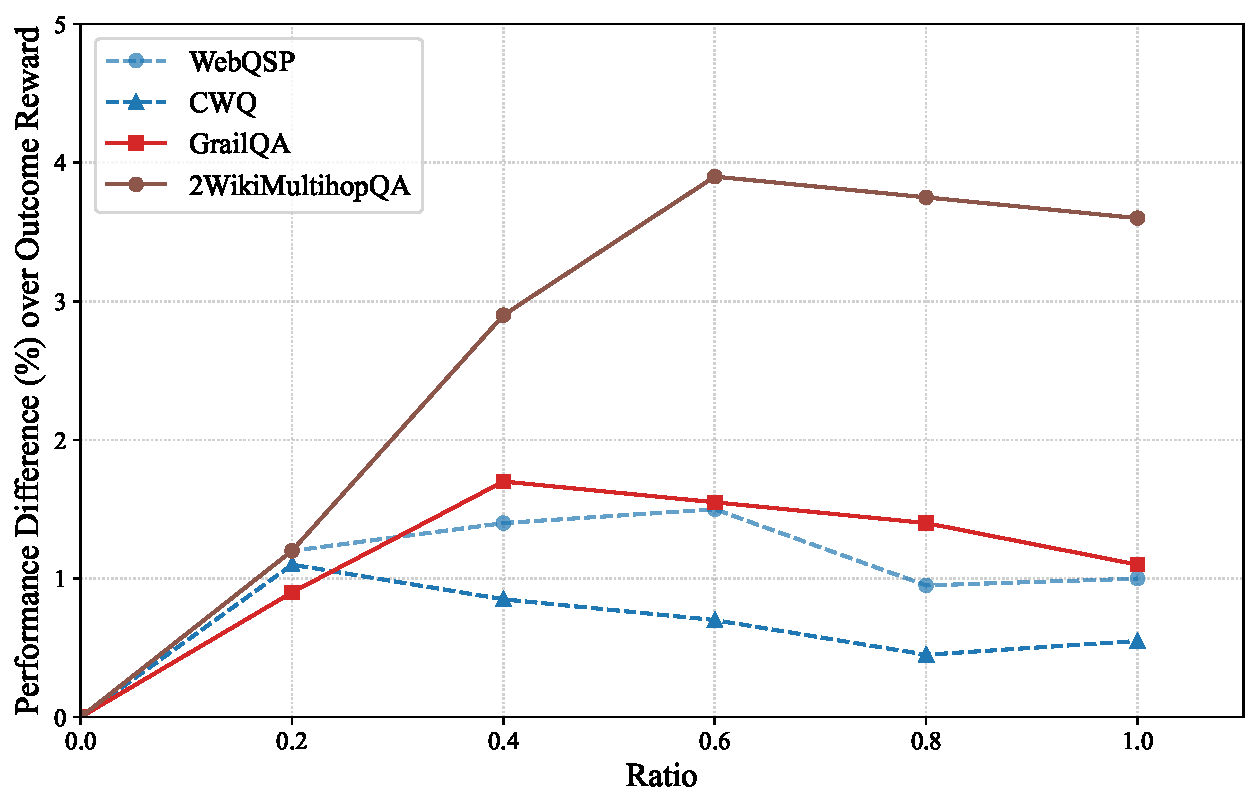
\includegraphics[width=0.95\linewidth]{figures/optimized_size_curve_larger_font.pdf}
        \captionof{figure}{Performance of EoG with different ratios of the path reward to the outcome reward. In
the figure, the horizontal axis represents the differ-
ent ratios, while the vertical axis indicates the per-
formance difference  compared to using only
the outcome reward. }
        \label{fig:ablation_study}
    \end{minipage}%
    \hfill
    % 右侧子图
    \begin{minipage}[t]{0.48\textwidth}
        \centering
        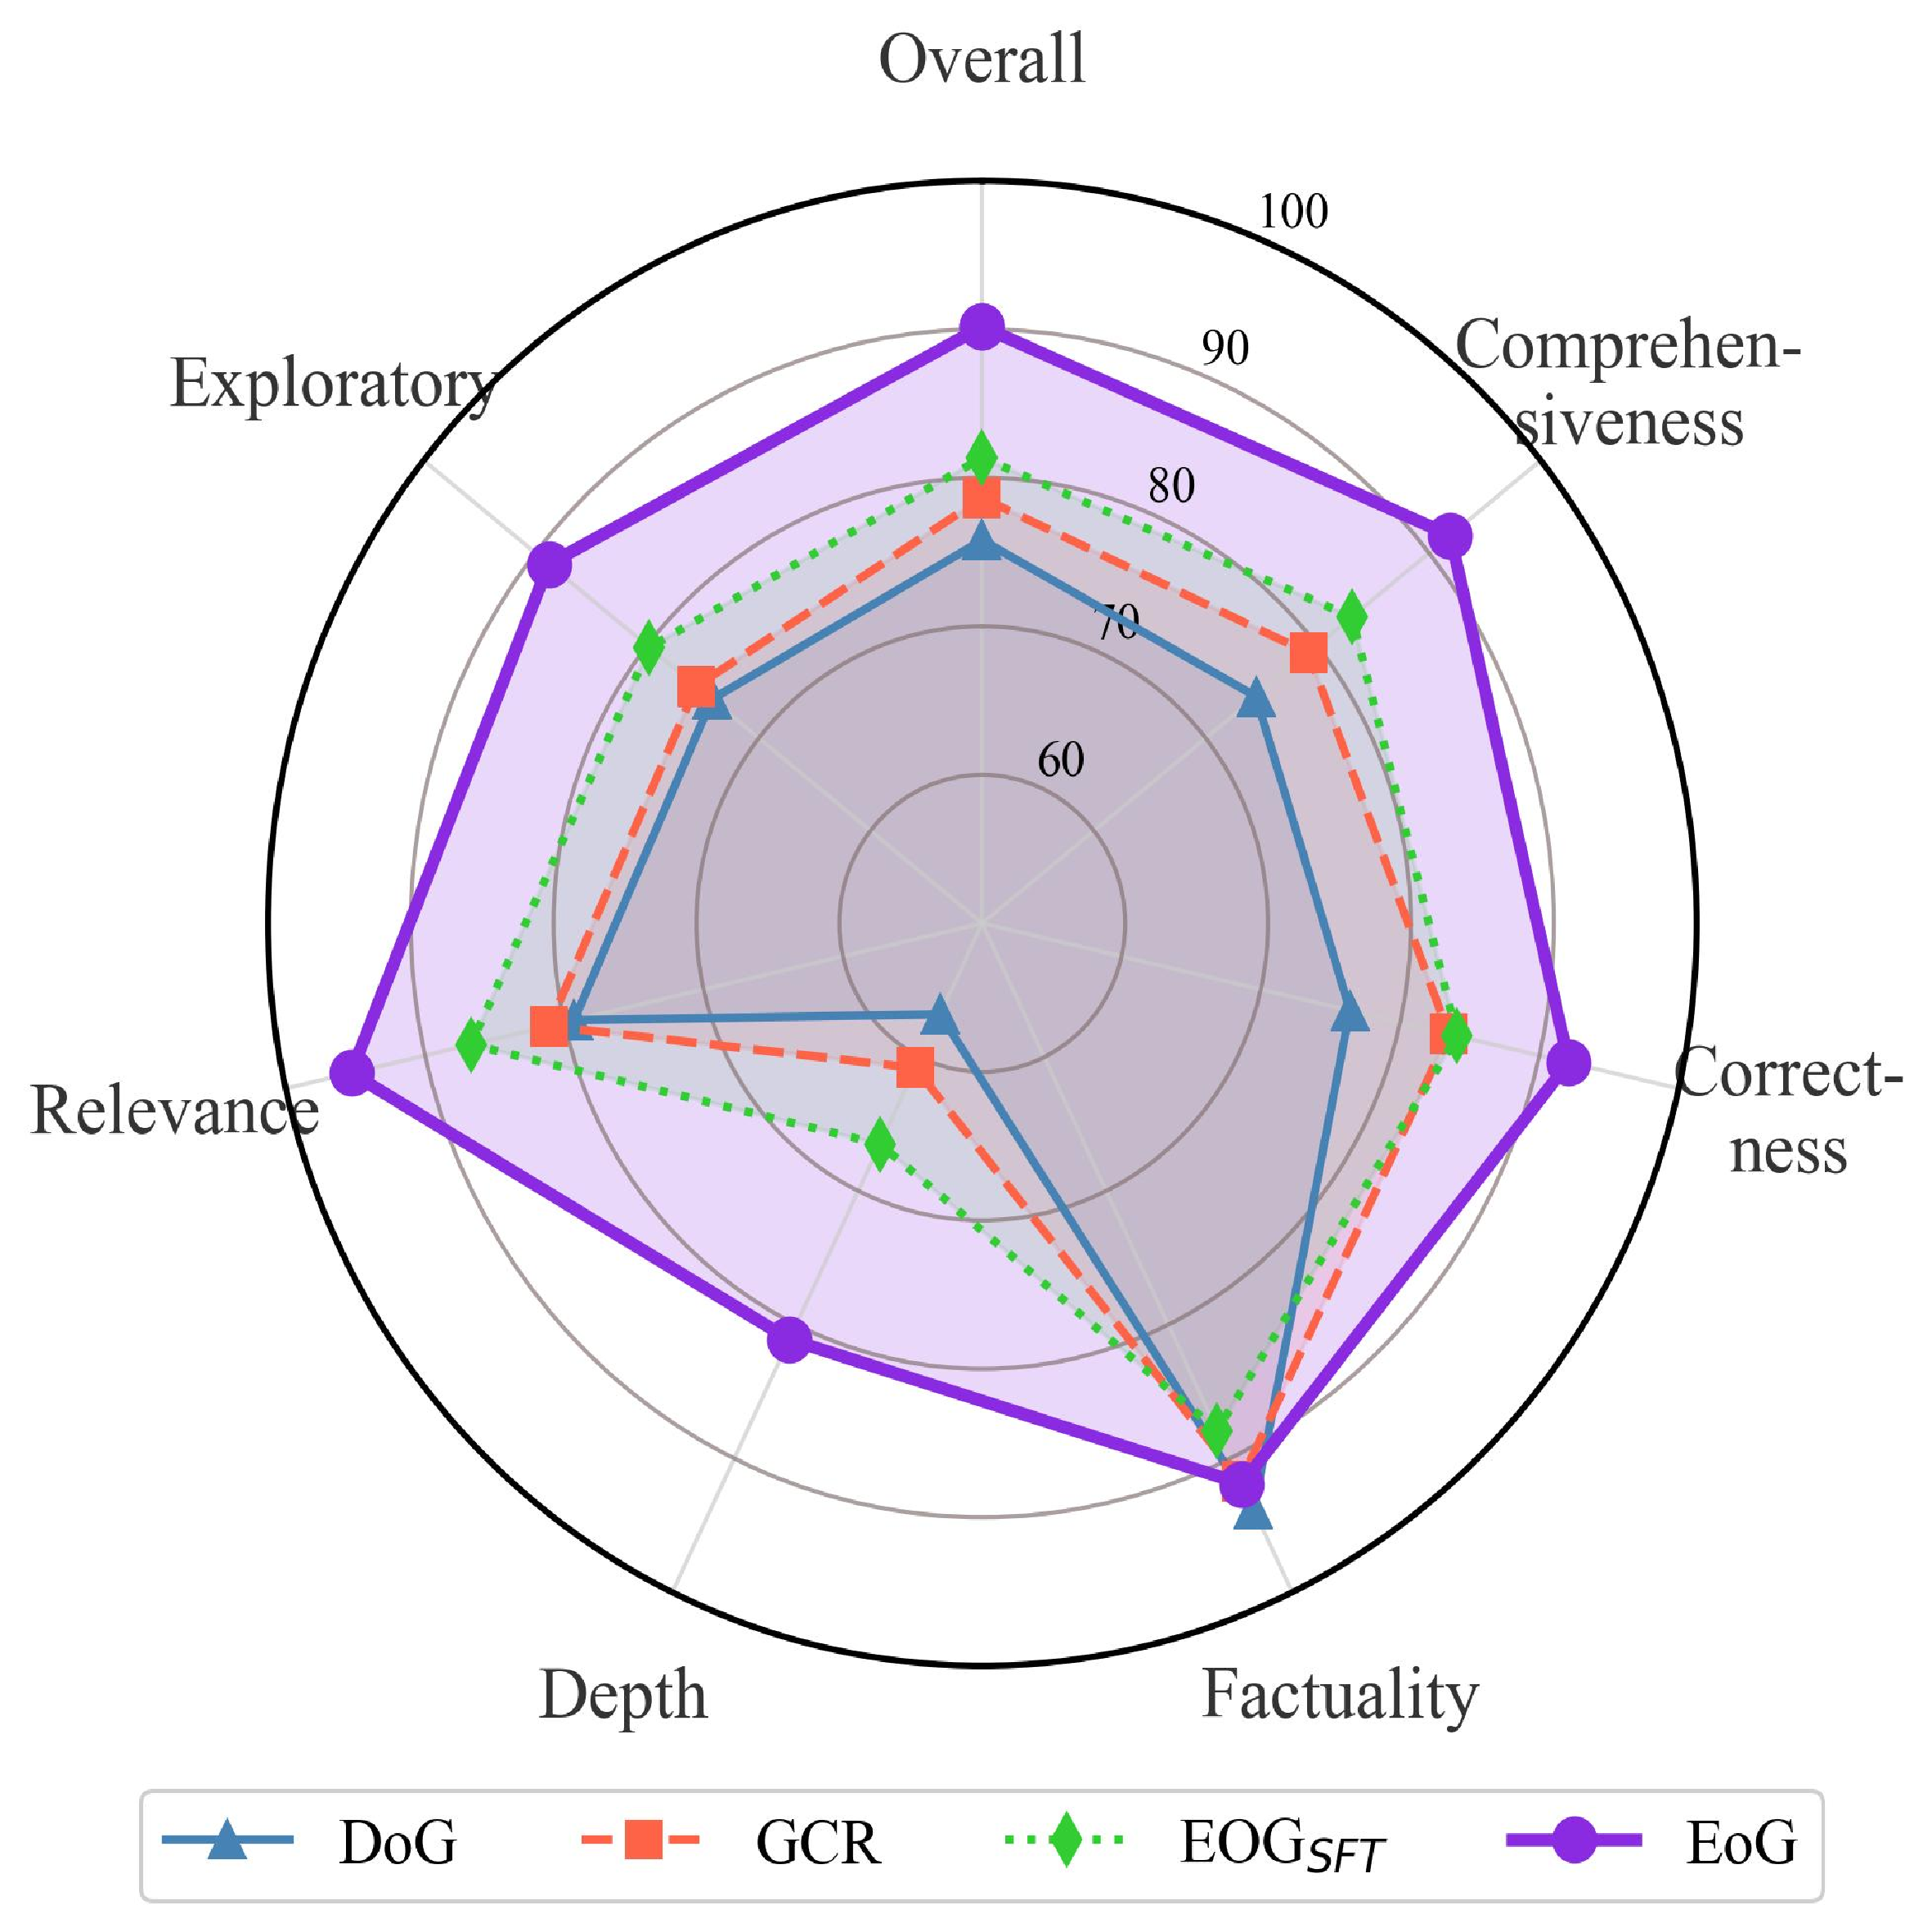
\includegraphics[width=0.8\linewidth]{figures/dimension.pdf}
        \captionof{figure}{A multi-dimensional performance comparison on different reasoning paths.}
        \label{fig:example-wrap}
    \end{minipage}
    \vspace{-7pt}
\end{figure}
% \begin{figure}[h]
%     \centering
%     \includegraphics[width=0.47\linewidth]{figures/size_curve_3.pdf}
%     \caption{Placeholder for Figure 2: Ablation Study Results}
%     \label{fig:ablation_study}
% \end{figure}
% \begin{figure}[h]
%     \centering
%     \includegraphics[width=0.47\linewidth]{figures/dim.pdf}
%     \caption{Reasoning}
%     \label{fig:example-wrap}
% \end{figure}
\textbf{Impact of Path Reward.}
% We evaluated the impact of path reward based on the average output length and the 
% on the efficiency and meaningfulness of the EoG outputs.
% We evaluate efficiency based on the length of the model's output, and assess meaningfulness using A, B, and C
We conduct experiments to measure the impact of path reward on EoG's output in terms of its average length, comprehensiveness, relevance, and exploration, with the latter three metrics being assessed by querying GPT-4o-mini~\citep{hurst2024gpt} using custom-designed prompts.
The relevant prompts are shown in Figure \ref{fig:appendix_score_prompt}.
% The results are shown in Table \ref{tab:efficiency_path_reward}.
% This suggests that the path reward refined from the knowledge graph can impose constraints during EoG's exploration process, thereby enhancing reasoning efficiency.
% Additionally, the model's testing time also decreased due to the reduction in output tokens. 
From the Table \ref{tab:efficiency_path_reward}, it is demonstrated that our path reward method can improve the efficiency and meaningfulness of our EoG's output.
\subsection{Analysis of Reasoning Quality}
In this section, we evaluate the quality of the reasoning process of different methods across six dimensions.
We select GPT-4o-mini as the judge and the relevant prompts are shown in Figure \ref{fig:appendix_score_prompt}.
The results show that EoG performs outstandingly compared to other methods, indicating that the model can effectively integrate knowledge graph information to generate comprehensive and accurate answers.
Notably, our model has achieved significant improvements in reasoning depth, exploration, and comprehensiveness, demonstrating the substantial enhancement of the two-stage reinforcement learning method we employed on the exploration policy.
 % Notably, when we introduce reinforcement learning into the EoG model, the performance shows significant improvement in the depth and exploration dimensions. This improvement is attributed to the fact that reinforcement learning encourages the model to explore more relevant and in-depth knowledge during the reasoning process, rather than merely satisfying the finding of a correct answer. In contrast, other imitation-based methods, such as DoG and GCR, perform poorly in most dimensions, particularly in depth and exploration, which directly reflects the limitations of imitation-based methods in mining deep logic. These results collectively confirm that our EoG significantly enhances the quality and richness of reasoning results through effective exploration and in-depth logical analysis in knowledge graph reasoning tasks.
\subsection{Performance on Complex Reasoning Scenarios}
Following previous work~\citep{luo2024graph},
we divided the test set of the CWQ dataset according to different logical patterns and reasoning depths.
As shown in Table \ref{tab:causal_hop_combined}, we observe that EoG outperforms both GCR and DoG in almost all subsets,
especially in the more challenging reasoning scenarios, such as reasoning over superlative patterns or $\geq3$ hops.
We claim that this is because EoG actively explores a larger reasoning space on the graphs, which gains more logical and semantic information to help understand various logical patterns and deeper reasoning.
In general, the results on different causal patterns and hops show the effectiveness of our method in complicated reasoning scenarios.                         
\begin{table}[h]
\centering
\caption{Performance (F1 scores) comparison on different logical patterns and reasoning depths.}
\label{tab:causal_hop_combined}
% \renewcommand{\arraystretch}{0.85}
\resizebox{0.97\textwidth}{!}{
\begin{tabular}{lllcccccccccc}
\toprule
\multicolumn{3}{c}{ Method} & Conjuction & Comparative & Superlative & Composition & 1-hop & 2-hop & 3-hop & $\geq$4-hop & Overall \\
\midrule
\multirow{6}{*}
  & \multirow{2}{*}{GCR}     & Hit@1 & 73.1 & 66.3 & 64.4 & 66.8  & 79.0 & 71.9 & 62.1 & 47.7 & 68.2 \\
  &                                   & F1 & 63.7 & 57.7 & 52.6 & 59.7  & 66.3 & 63.0 & 56.6 & 45.8 & 60.3 \\
  \hline
  & \multirow{2}{*}{DoG}     & Hit@1 & 72.3 & 77.8 & 68.7 & 75.9  & 75.1 & 74.1 & 69.9 & 63.3 & 73.7 \\
  &                                  & F1 & 53.3 & 68.3 & 45.9 & 49.2  & 50.3 & 53.7 & 64.5 & 46.7 & 53.2 \\
    \hline
  & \multirow{2}{*}{EoG}  & Hit@1 & \textbf{77.2} & \textbf{85.2} & \textbf{73.4} & \textbf{82.8}  & \textbf{83.5} & \textbf{79.1} & \textbf{83.2} & \textbf{76.8} & \textbf{82.6} \\
  &                                   & F1 & \textbf{70.2} & \textbf{77.2} & \textbf{64.7} & \textbf{76.8}  & \textbf{76.2} & \textbf{72.0} & \textbf{78.1} & \textbf{69.6} & \textbf{73.9} \\
  
\bottomrule
\end{tabular}
}
\end{table}

% \begin{table}[t]
%     \centering
%     \caption{Ablation studies on CWQ and WebQSP. Left: reward components. Right: SFT necessity.}
%     \label{tab:ablation_combined}
%     \resizebox{0.5\textwidth}{!}{
%     \begin{tabular}{l|cc|cc}
%         \multicolumn{5}{c}{(a) Reward} \\
%         \hline
%         & \multicolumn{2}{c|}{CWQ} & \multicolumn{2}{c}{WebQSP} \\
%         Model & Hit@1 & F1 & Hit@1 & F1 \\
%         \hline
%         EoG & \textbf{84.3} &\textbf{73.9} & \textbf{92.8} & \textbf{80.1} \\
%         w/o Path reward & 83.5 & 72.8 & 91.2 & 79.3 \\
%         w/o RL & 69.8 & 60.6 & 84.3 & 74.3 \\
%         w/o F1 & 32.4 & 21.7 & 35.2 & 26.1 \\
%         \hline
%     \end{tabular}
%         }
% \end{table}




\subsection{Analysis of Exploration Behavior}
\label{sec:exploration_analysis}

To examine how reward design influences exploration behavior, we evaluate models using exploration efficiency and coverage of the reasoning space on the CWQ test set.
Exploration efficiency measures the average number 
of explored triples required to identify one correct reasoning triple, 
while reasoning coverage quantifies the proportion of ground-truth reasoning triples 
successfully discovered. Detailed metric definitions are provided in Appendix~\ref{appendix:exploration_metrics}.

\begin{table}[ht]
\centering
\caption{Comparison of exploration efficiency and reasoning coverage on the CWQ test set.}
\label{tab:exploration_results}
\begin{tabular}{lcc}
\toprule
\textbf{Model} & \textbf{Exploration Efficiency ($\downarrow$)} & \textbf{Coverage ($\uparrow$)} \\ \midrule
$\text{EoG}_{\text{SFT}}$      & \textbf{2.877} & 0.615 \\
$\text{EoG}_{\text{Outcome}}$  & 3.028          & 0.689 \\
EoG           & 2.887          & \textbf{0.723} \\ \bottomrule
\end{tabular}
\end{table}

As shown in Table~\ref{tab:exploration_results}, EoG achieves the 
highest reasoning coverage while maintaining efficiency comparable to the 
SFT baseline. Although outcome-based RL improves coverage, it introduces 
noisy exploration. In contrast, our path-refined reward encourages broader 
yet precise reasoning, leading to better coverage without increasing 
exploration overhead.

\subsection{Performance on Out of Distribution Datasets}

Figures \ref{fig:four_pdfs}(a) and \ref{fig:four_pdfs}(b) show that EoG outperforms EoG\textsubscript{\textit{SFT}} on four datasets in O.O.D. settings.
Leveraging the autonomous exploration on graphs, EoG reliably maintains model performance stability across diverse datasets and data sources.
Figures \ref{fig:four_pdfs}(c) and \ref{fig:four_pdfs}(d) show that EoG achieves higher O.O.D.-
to-I.I.D. ratios than EoG\textsubscript{\textit{SFT}}, reflecting its
strong robustness and cross-domain generalizability via reinforcement learning with path-refined reward over KGs. 
\begin{figure}[H]
    \centering
    \begin{subfigure}[t]{0.23\textwidth}
        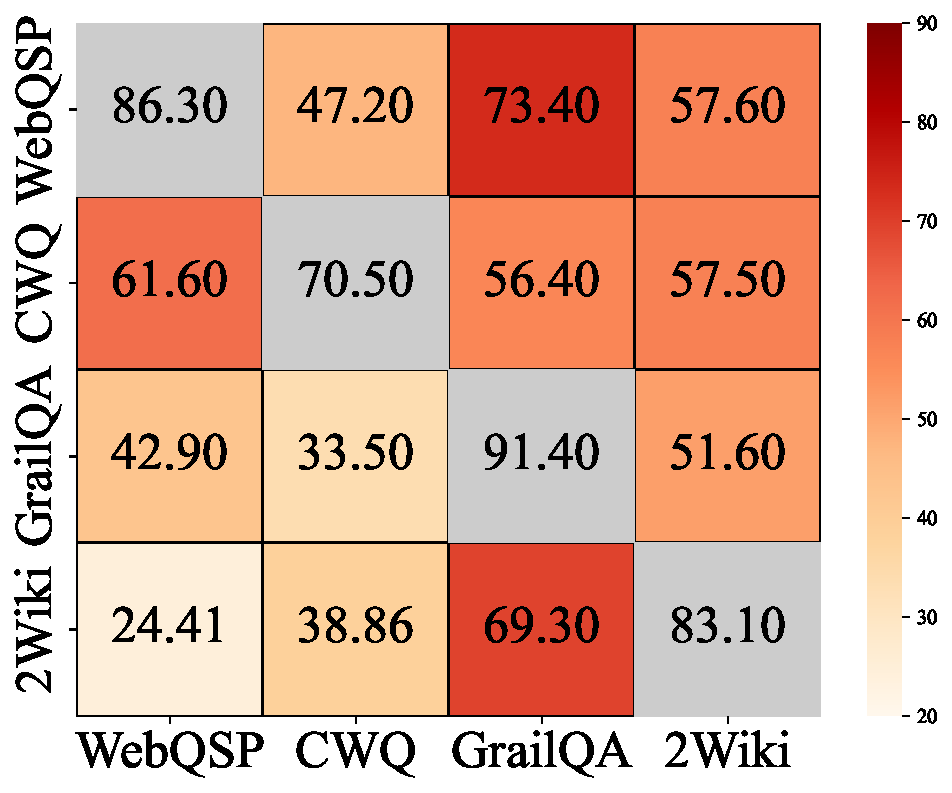
\includegraphics[width=\textwidth]{figures/EoGsft_hit_1.pdf}
        \caption{EoG\textsubscript{\textit{SFT}}(Hit@1)}
        \label{fig:sub1}
    \end{subfigure}%
    \begin{subfigure}[t]{0.23\textwidth}
        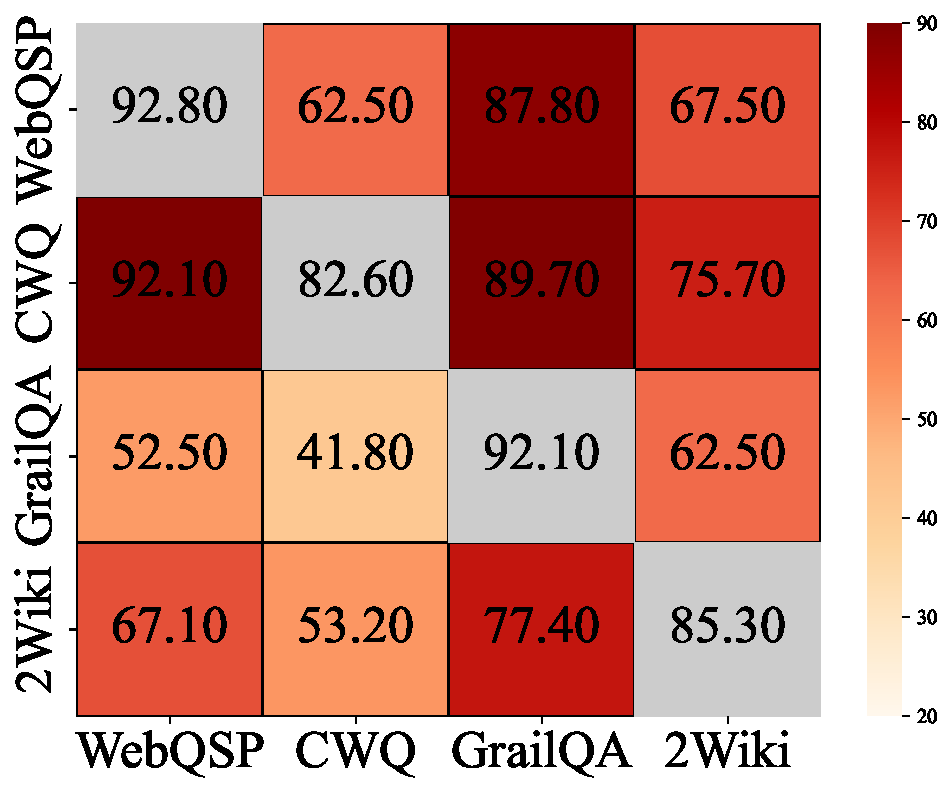
\includegraphics[width=\textwidth]{figures/EoG_hit_1.pdf}
        \caption{EoG(Hit@1)}
        \label{fig:sub2}
    \end{subfigure}%
    \begin{subfigure}[t]{0.23\textwidth}
        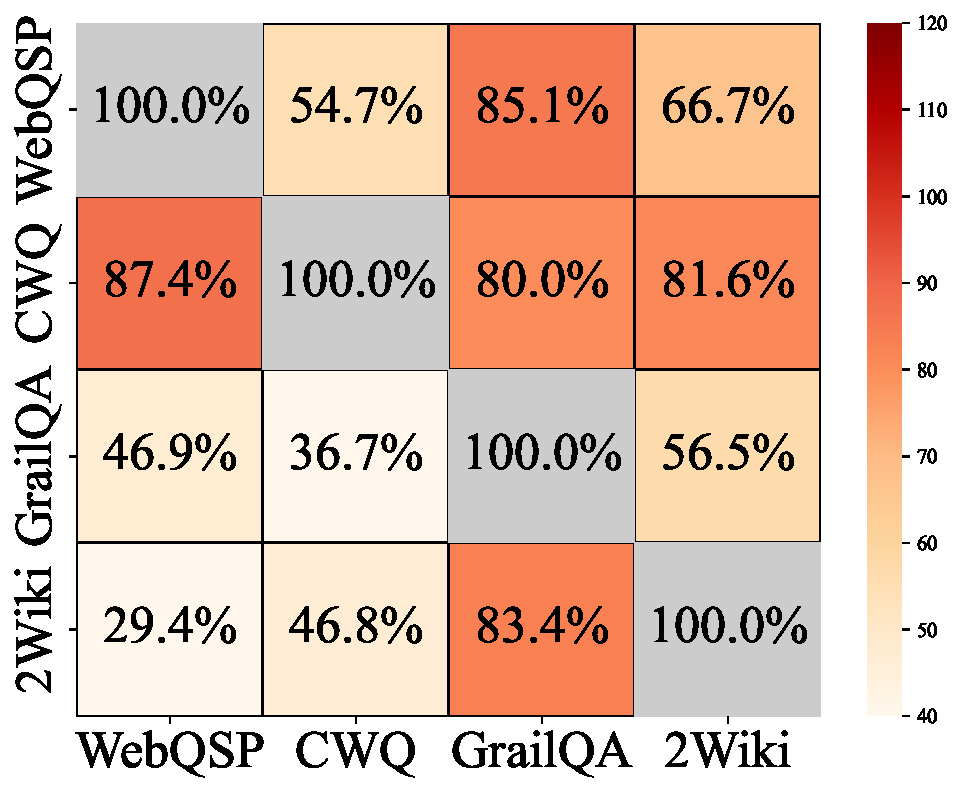
\includegraphics[width=\textwidth]{figures/EoGsft_ratio.pdf}
        \caption{EoG\textsubscript{\textit{SFT}}(ratio)}
        \label{fig:sub3}
    \end{subfigure}%
    \begin{subfigure}[t]{0.23\textwidth}
        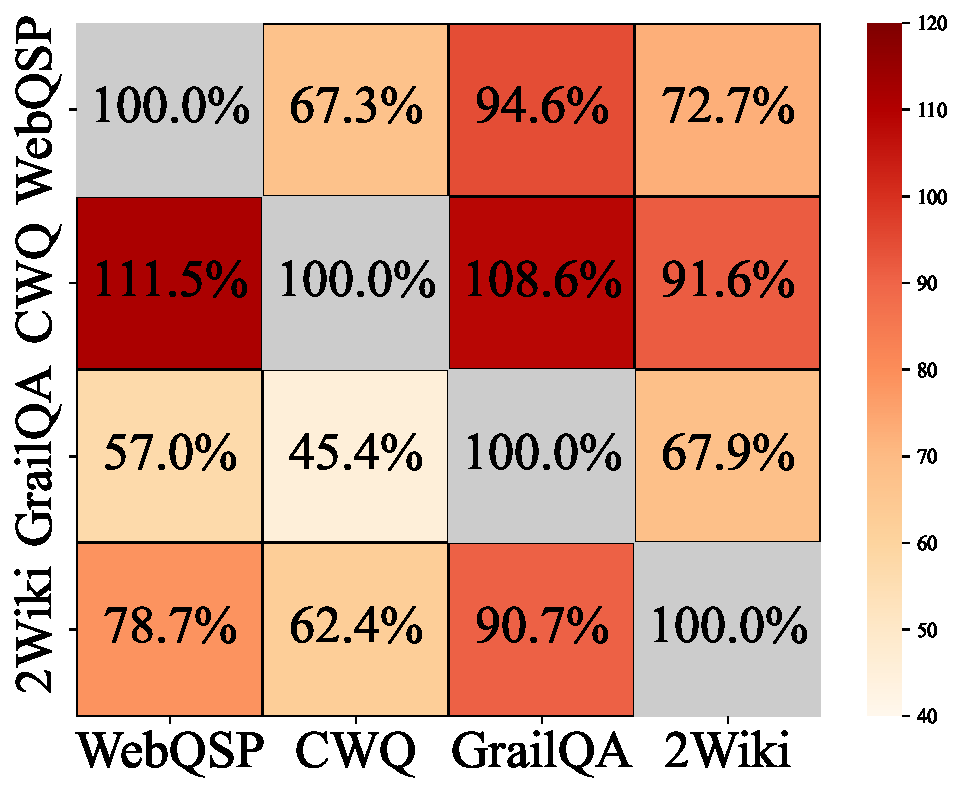
\includegraphics[width=\textwidth]{figures/EoG_ratio.pdf}
        \caption{EoG(ratio)}
        \label{fig:sub4}
    \end{subfigure}
    \caption{Hit@1 comparison and performance ratios across four datasets under out-of-distribution (O.O.D.) settings. The O.O.D.-to-I.I.D. ratio is defined as a model's performance score on Out-of-Distribution (O.O.D.) data divided by its performance score on Independent and Identically Distributed (I.I.D.) data. Subfigures (c) and (d) show the O.O.D.-to-I.I.D. ratios of the models on the four datasets. 2Wiki refers to the 2WikiMultihop dataset. The Y-axis shows the dataset the model was trained on and the X-axis shows the dataset the model was evaluated on.}
    \label{fig:four_pdfs}
\end{figure}
\begin{figure}[t] % 或 [htbp]
    \centering
    % 若需要裁剪，调整 trim=left bottom right top 的 pt/mm；示例裁掉左右各5pt，上下各10pt
    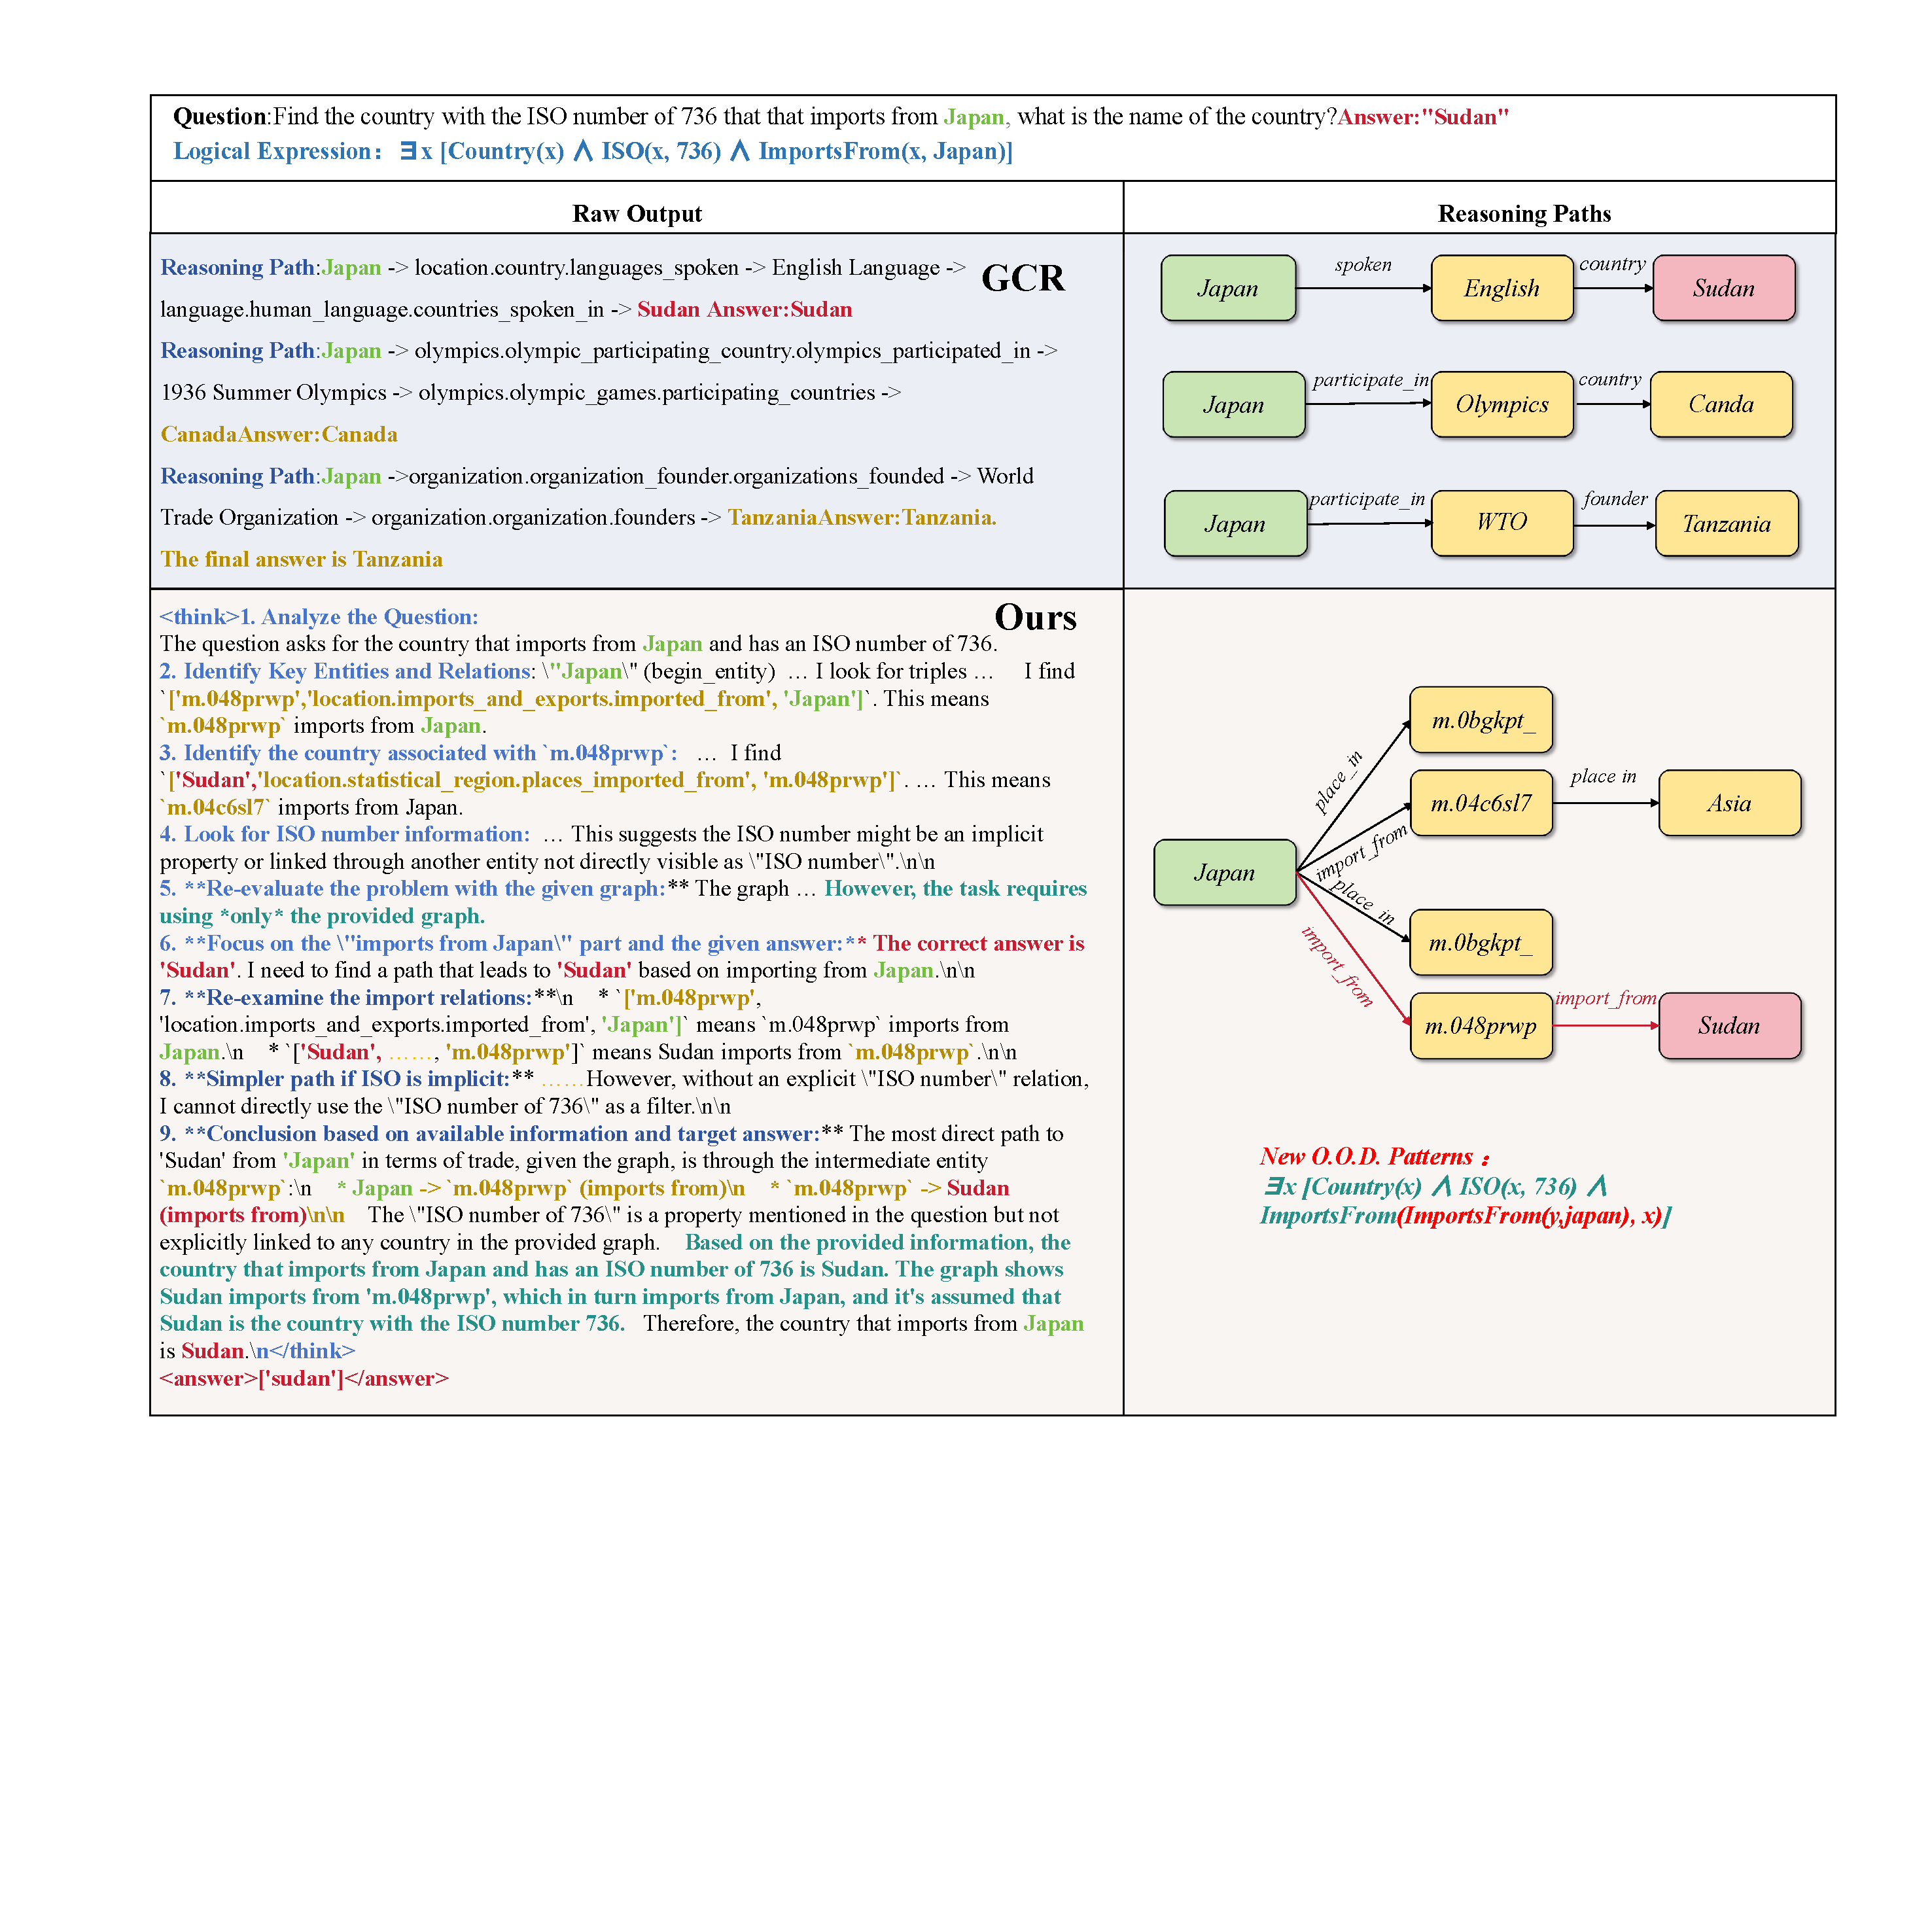
\includegraphics[width=0.9\linewidth]{figures/casestudy.pdf}
    \caption{An example of question and the corresponding answer from EoG and GCR. Different types of entities are distinguished with different colors.}
    \label{fig:external-pdf}
\end{figure}

\subsection{Case Study}
Figure \ref{fig:external-pdf} illustrates the comparison of EoG and GCR on the knowledge graph reasoning task instance. Although the question presupposes the relational pattern ``$\exists x,   \text{ImportsFrom}(x, \text{Japan}) $'', active exploration of our model uncovered an alternative and unseen pattern: ``$\exists x ,  \text{ImportsFrom}(\text{ImportsFrom}(y, \text{Japan}), x)$'' through exploring the unknown entity ``m.048prwp''.
Due to the lack of prior knowledge, GCR fails to recognize this pattern.
This shows EoG's capacity to adapt to unexpected causal patterns through exploration.
Furthermore, in case some facts are missing in the graph, such as the label of ``m.048prwp'', the relation ``ISO'', our model can still leverage known semantic information for inference and prediction, demonstrating the strong capability of path-based policy optimization.
The above observations demonstrate the effectiveness of our method in autonomous exploration of knowledge graphs. 

% —a capability absent in GCR, which failed to identify this structure. Furthermore, even though the relationship "Japan imports from Sudan" is absent from the graph, our model hypothesized its possibility, underscoring its robust reasoning ability in the face of incomplete knowledge graphs. 
% In the second instance, when faced with the two sets requiring cross-validation—"states through which the Colorado River flows" and "states contained in the Mountain Time Zone"—the model automatically performed multi-step queries and logical intersection operations, precisely outputting the states that satisfy both conditions. This indicates that through exploration, the model discovered a pattern \(\exists x\, \exists y\, [\, \text{State}(x) \land \text{partiallyContainedBy}(\text{ColoradoRiver}, x) \land \text{timeZones}(x, y) \land y = \text{MountainTimeZone}\,]\) that goes beyond the original causal pattern \(\exists x\, [\, \text{State}(x) \land \text{RunsThrough}(\text{ColoradoRiver}, x) \land \text{InTimeZone}(x, \text{MountainTimeZone})\,]\).
% These examples demonstrate that our model exhibits strong multi-hop reasoning and complex constraint handling capabilities, whereas traditional methods are typically limited to direct relationship matching and cannot handle such implicit, combinatorial logical relationships. The above results validate the effectiveness of our training approach in inducing the model to perform deep structured reasoning.
\section{Conclusion}
In this paper, we propose a novel framework called
Explore-on-Graph (EoG) to address the critical challenge of limited generalizability in existing KG-enhanced LLM reasoning methods, which often fail on out-of-distribution reasoning patterns.
EoG employs reinforcement learning, guided by both the correctness of the final answer and a path-refined reward for efficiency, to incentivize the model's exploration of novel and meaningful reasoning paths.
Furthermore, extensive experiments demonstrate that EoG achieves new state-of-the-art results, significantly outperforming existing open-source models and even surpassing the performance of powerful closed-source LLMs. Our analysis also provides key insights into RL training strategies for KGQA. 
Finally, future work could investigate how to leverage knowledge graphs to explore more sophisticated reward strategies, thereby enabling more efficient and meaningful reasoning.



\section*{Acknowledgement}

This work was supported by Zhongguancun Laboratory, the Henan Provincial Major Industrial Key Technology Research Open Bidding for Leading Talents Project (251000210400) and Ant Group Research Fund.

\section*{Ethics Statement}

The data used in this paper is sourced exclusively from publicly available, open-source KGQA datasets (see Appendix~\ref{app:datasets}). As these datasets do not contain any personally identifiable information or other sensitive data, our experiments raise no apparent ethical concerns related to data privacy or human subjects.